\documentclass{standalone}
\usepackage{tikz}
\usetikzlibrary{patterns, positioning}
\usepackage[sfdefault]{ClearSans} %% option 'sfdefault' activates Clear Sans as the default text font
\usepackage[T1]{fontenc}

\begin{document}
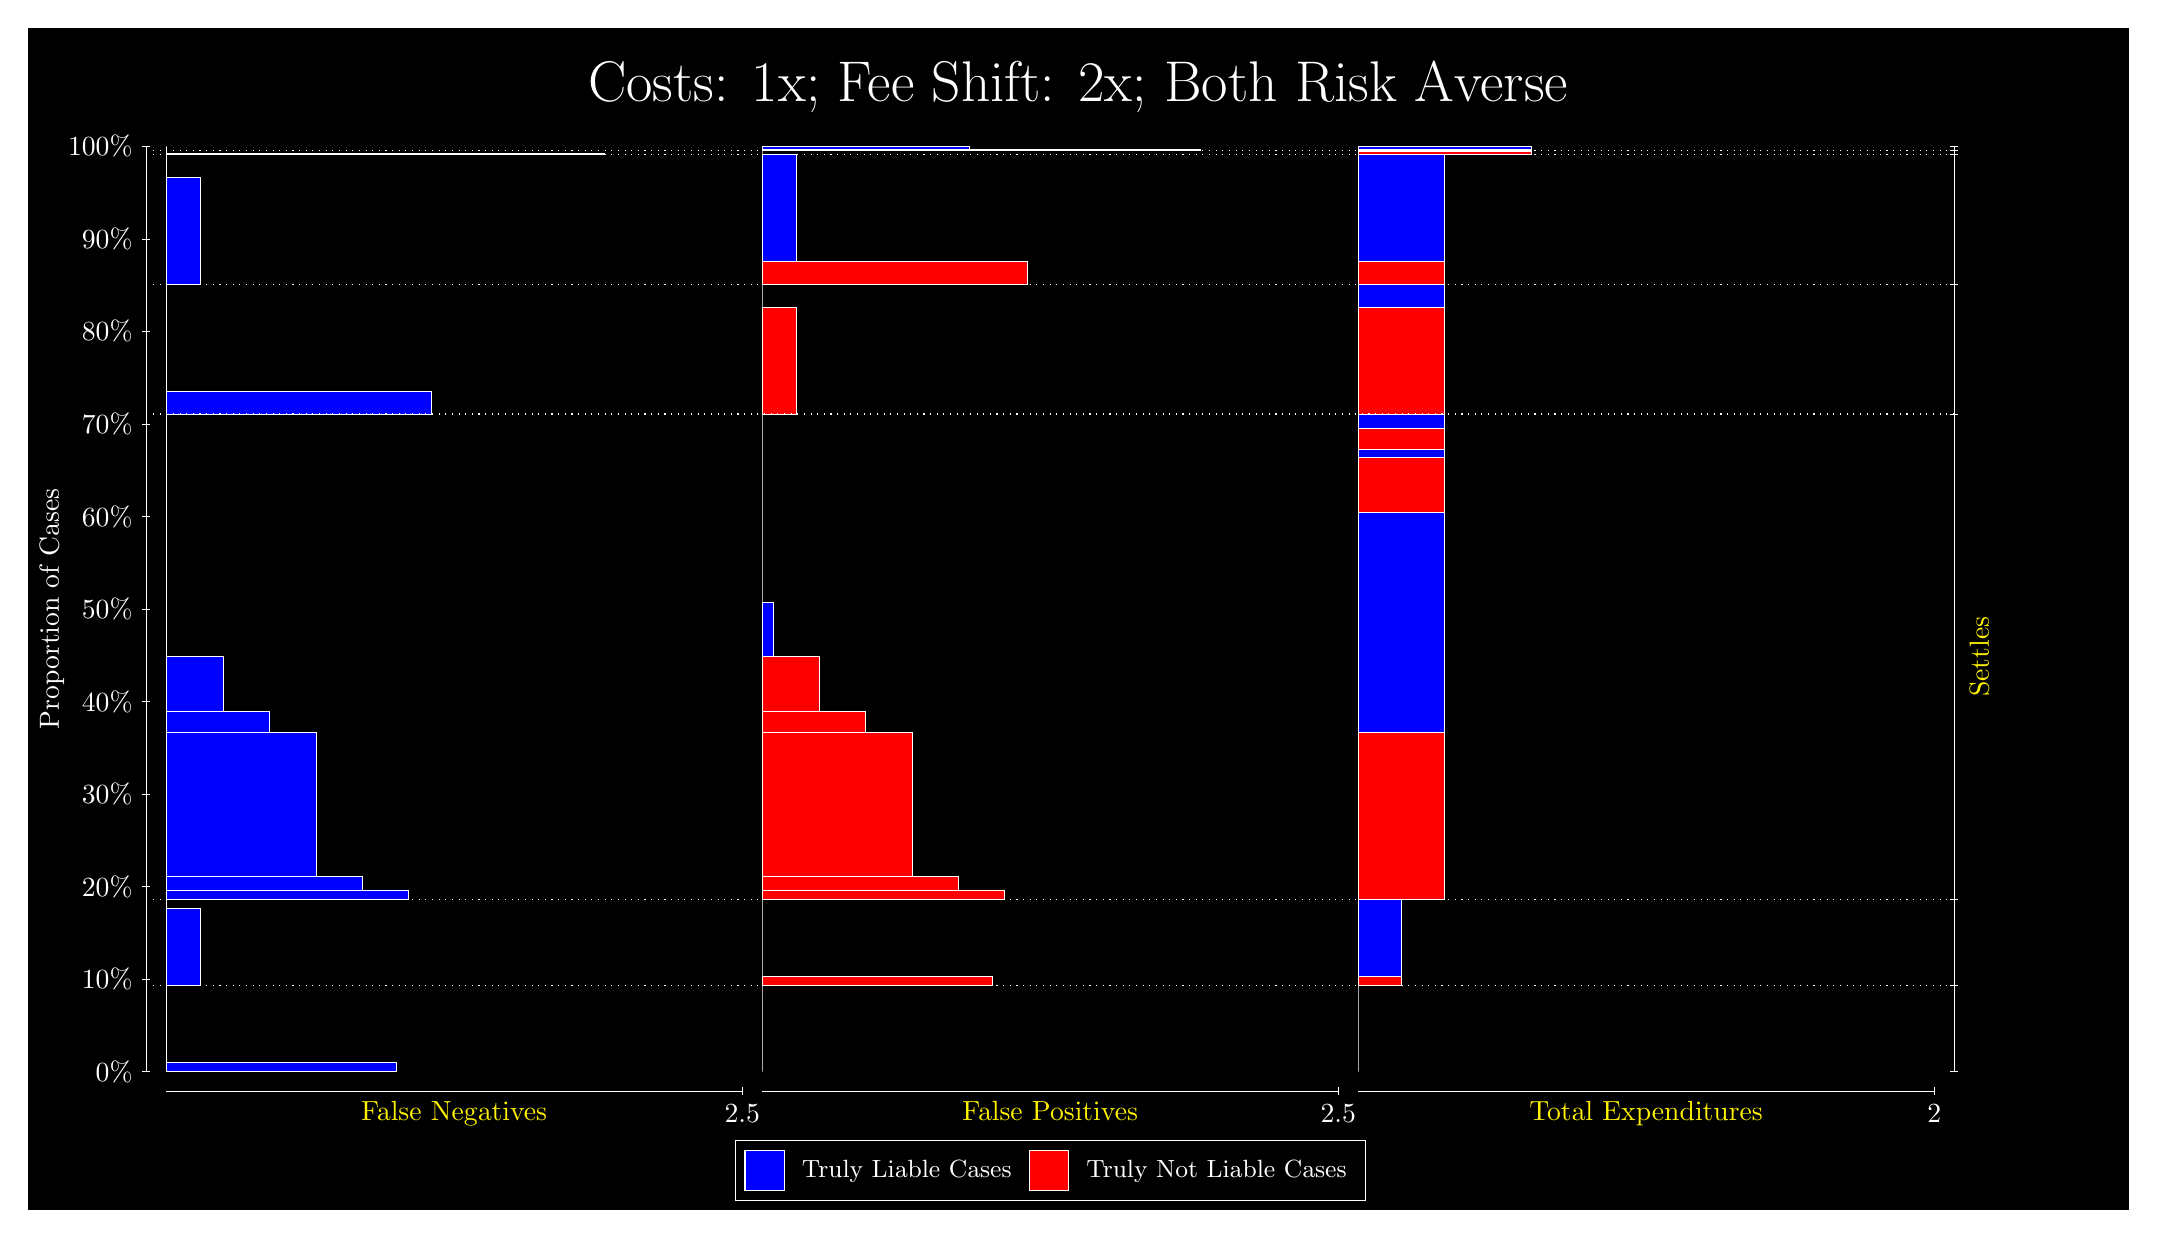
\begin{tikzpicture}
\draw[fill=black] (0,0) rectangle (26.667,15);
\draw[text=white] (0,13.5) rectangle (26.667,15) node[midway] {\huge Costs: 1x; Fee Shift: 2x; Both Risk Averse};
\draw[white, very thin] (1.5,1.75) -- (1.5,13.5);
\node[rotate=90, text=white, anchor=center] at (0.3, 7.625) {Proportion of Cases};
\draw[white, very thin] (1.45,1.75) -- (1.55,1.75);
\node[text=white, anchor=east] at (1.45, 1.75) {0\%};
\draw[white, very thin] (1.45,2.925) -- (1.55,2.925);
\node[text=white, anchor=east] at (1.45, 2.925) {10\%};
\draw[white, very thin] (1.45,4.1) -- (1.55,4.1);
\node[text=white, anchor=east] at (1.45, 4.1) {20\%};
\draw[white, very thin] (1.45,5.275) -- (1.55,5.275);
\node[text=white, anchor=east] at (1.45, 5.275) {30\%};
\draw[white, very thin] (1.45,6.45) -- (1.55,6.45);
\node[text=white, anchor=east] at (1.45, 6.45) {40\%};
\draw[white, very thin] (1.45,7.625) -- (1.55,7.625);
\node[text=white, anchor=east] at (1.45, 7.625) {50\%};
\draw[white, very thin] (1.45,8.8) -- (1.55,8.8);
\node[text=white, anchor=east] at (1.45, 8.8) {60\%};
\draw[white, very thin] (1.45,9.975) -- (1.55,9.975);
\node[text=white, anchor=east] at (1.45, 9.975) {70\%};
\draw[white, very thin] (1.45,11.15) -- (1.55,11.15);
\node[text=white, anchor=east] at (1.45, 11.15) {80\%};
\draw[white, very thin] (1.45,12.325) -- (1.55,12.325);
\node[text=white, anchor=east] at (1.45, 12.325) {90\%};
\draw[white, very thin] (1.45,13.5) -- (1.55,13.5);
\node[text=white, anchor=east] at (1.45, 13.5) {100\%};

\draw[white, very thin] (24.457,1.75) -- (24.457,13.5);
\draw[white, very thin] (24.407,1.75) -- (24.507,1.75);
\node[anchor=west] at (24.407, 1.75) {};
\draw[white, very thin] (24.407,2.8432) -- (24.507,2.8432);
\node[anchor=west] at (24.407, 2.8432) {};
\draw[white, very thin] (24.407,3.9362) -- (24.507,3.9362);
\node[anchor=west] at (24.407, 3.9362) {};
\draw[white, very thin] (24.407,10.1) -- (24.507,10.1);
\node[anchor=west] at (24.407, 10.1) {};
\draw[white, very thin] (24.407,11.749) -- (24.507,11.749);
\node[anchor=west] at (24.407, 11.749) {};
\draw[white, very thin] (24.407,13.398) -- (24.507,13.398);
\node[anchor=west] at (24.407, 13.398) {};
\draw[white, very thin] (24.407,13.449) -- (24.507,13.449);
\node[anchor=west] at (24.407, 13.449) {};
\draw[white, very thin] (24.407,13.5) -- (24.507,13.5);
\node[anchor=west] at (24.407, 13.5) {};

\draw[white, very thin, fill=blue] (1.75,1.75) rectangle (4.6775,1.865);
\draw[white, very thin, fill=red] (1.75,1.865) rectangle (1.75,2.8432);
\draw[white, very thin, fill=blue] (1.75,2.8432) rectangle (2.1891,3.8212);
\draw[white, very thin, fill=red] (1.75,3.8212) rectangle (1.75,3.9362);
\draw[white, very thin, fill=blue] (1.75,3.9362) rectangle (4.8239,4.0463);
\draw[white, very thin, fill=blue] (1.75,4.0463) rectangle (4.2384,4.2242);
\draw[white, very thin, fill=blue] (1.75,4.2242) rectangle (3.6529,6.0581);
\draw[white, very thin, fill=blue] (1.75,6.0581) rectangle (3.0674,6.3225);
\draw[white, very thin, fill=blue] (1.75,6.3225) rectangle (2.4819,7.018);
\draw[white, very thin, fill=red] (1.75,7.018) rectangle (1.75,10.1);
\draw[white, very thin, fill=blue] (1.75,10.1) rectangle (5.1167,10.388);
\draw[white, very thin, fill=red] (1.75,10.388) rectangle (1.75,11.749);
\draw[white, very thin, fill=blue] (1.75,11.749) rectangle (2.1891,13.11);
\draw[white, very thin, fill=red] (1.75,13.11) rectangle (1.75,13.398);
\draw[white, very thin, fill=blue] (1.75,13.398) rectangle (7.3123,13.415);
\draw[white, very thin, fill=red] (1.75,13.415) rectangle (1.75,13.449);
\draw[white, very thin, fill=red] (1.75,13.449) rectangle (1.75,13.466);
\draw[white, very thin, fill=blue] (1.75,13.466) rectangle (1.75,13.5);
\draw[white, very thin, fill=red] (9.3189,1.75) rectangle (9.3189,2.7282);
\draw[white, very thin, fill=blue] (9.3189,2.7282) rectangle (9.3189,2.8432);
\draw[white, very thin, fill=red] (9.3189,2.8432) rectangle (12.246,2.9582);
\draw[white, very thin, fill=blue] (9.3189,2.9582) rectangle (9.3189,3.9362);
\draw[white, very thin, fill=red] (9.3189,3.9362) rectangle (12.393,4.0463);
\draw[white, very thin, fill=red] (9.3189,4.0463) rectangle (11.807,4.2242);
\draw[white, very thin, fill=red] (9.3189,4.2242) rectangle (11.222,6.0582);
\draw[white, very thin, fill=red] (9.3189,6.0582) rectangle (10.636,6.3225);
\draw[white, very thin, fill=red] (9.3189,6.3225) rectangle (10.051,7.018);
\draw[white, very thin, fill=blue] (9.3189,7.018) rectangle (9.4652,7.7136);
\draw[white, very thin, fill=blue] (9.3189,7.7136) rectangle (9.3189,10.1);
\draw[white, very thin, fill=red] (9.3189,10.1) rectangle (9.758,11.461);
\draw[white, very thin, fill=blue] (9.3189,11.461) rectangle (9.3189,11.749);
\draw[white, very thin, fill=red] (9.3189,11.749) rectangle (12.686,12.037);
\draw[white, very thin, fill=blue] (9.3189,12.037) rectangle (9.758,13.398);
\draw[white, very thin, fill=red] (9.3189,13.398) rectangle (9.3189,13.432);
\draw[white, very thin, fill=blue] (9.3189,13.432) rectangle (9.3189,13.449);
\draw[white, very thin, fill=red] (9.3189,13.449) rectangle (14.881,13.466);
\draw[white, very thin, fill=blue] (9.3189,13.466) rectangle (11.954,13.5);
\draw[white, very thin, fill=red] (16.888,1.75) rectangle (16.888,2.7282);
\draw[white, very thin, fill=blue] (16.888,2.7282) rectangle (16.888,2.8432);
\draw[white, very thin, fill=red] (16.888,2.8432) rectangle (17.437,2.9582);
\draw[white, very thin, fill=blue] (16.888,2.9582) rectangle (17.437,3.9362);
\draw[white, very thin, fill=red] (16.888,3.9362) rectangle (17.986,6.0582);
\draw[white, very thin, fill=blue] (16.888,6.0582) rectangle (17.986,8.852);
\draw[white, very thin, fill=red] (16.888,8.852) rectangle (17.986,9.5475);
\draw[white, very thin, fill=blue] (16.888,9.5475) rectangle (17.986,9.6576);
\draw[white, very thin, fill=red] (16.888,9.6576) rectangle (17.986,9.9219);
\draw[white, very thin, fill=blue] (16.888,9.9219) rectangle (17.986,10.1);
\draw[white, very thin, fill=red] (16.888,10.1) rectangle (17.986,11.461);
\draw[white, very thin, fill=blue] (16.888,11.461) rectangle (17.986,11.749);
\draw[white, very thin, fill=red] (16.888,11.749) rectangle (17.986,12.037);
\draw[white, very thin, fill=blue] (16.888,12.037) rectangle (17.986,13.398);
\draw[white, very thin, fill=red] (16.888,13.398) rectangle (19.083,13.432);
\draw[white, very thin, fill=blue] (16.888,13.432) rectangle (19.083,13.449);
\draw[white, very thin, fill=red] (16.888,13.449) rectangle (19.083,13.466);
\draw[white, very thin, fill=blue] (16.888,13.466) rectangle (19.083,13.5);
\draw[white, dotted] (1.5,2.8432) -- (24.457,2.8432);
\draw[white, dotted] (1.5,3.9362) -- (24.457,3.9362);
\draw[white, dotted] (1.5,10.1) -- (24.457,10.1);
\draw[white, dotted] (1.5,11.749) -- (24.457,11.749);
\draw[white, dotted] (1.5,13.398) -- (24.457,13.398);
\draw[white, dotted] (1.5,13.449) -- (24.457,13.449);
\draw[white, very thin] (1.75,1.5) -- (9.0689,1.5);
\node[text=yellow, anchor=north] at (5.4094, 1.5) {False Negatives};
\draw[white, very thin] (9.0689,1.45) -- (9.0689,1.55);
\node[text=white, anchor=north] at (9.0689, 1.45) {2.5};

\draw[white, very thin] (9.3189,1.5) -- (16.638,1.5);
\node[text=yellow, anchor=north] at (12.978, 1.5) {False Positives};
\draw[white, very thin] (16.638,1.45) -- (16.638,1.55);
\node[text=white, anchor=north] at (16.638, 1.45) {2.5};

\draw[white, very thin] (16.888,1.5) -- (24.207,1.5);
\node[text=yellow, anchor=north] at (20.547, 1.5) {Total Expenditures};
\draw[white, very thin] (24.207,1.45) -- (24.207,1.55);
\node[text=white, anchor=north] at (24.207, 1.45) {2};



\node[text=yellow, centered, rotate=90] at (24.777, 7.018) {Settles};





\draw (12.978300999999998,1.5) node[draw=none] (baseCoordinate) {};
\begin{scope}[align=center]
        \matrix[scale=0.5, draw=white, below=0.5cm of baseCoordinate, nodes={draw}, column sep=0.1cm]{
            \node[rectangle, draw, minimum width=0.5cm, minimum height=0.5cm, fill=blue] {}; &
            \node[draw=none, font=\small, text=white] (B) {Truly Liable Cases}; &
            \node[rectangle, draw, minimum width=0.5cm, minimum height=0.5cm, fill=red] {}; &
            \node[draw=none, font=\small, text=white] (B) {Truly Not Liable Cases}; \\
            };
\end{scope}

\end{tikzpicture}
\end{document}